% siminos/atlas/intro.tex  pdflatex atlas
% $Author$ $Date$

\begin{quotation}
{\color{red}When they are writing down equations to describe a system, physicists try to take advantage
any symmetries presented by the problem at hand. While symmetries can greatly simplify
the mathematics and lead to elegant solutions, Nature does not respect them. 
Chaotic systems tend to break symmetries, even when the governing equations are symmetric.
Various methods exist to 'quotient out' symmetries in low-dimensional systems and thus address
important dynamical questions even in the presecence of symmetry breaking. However, 
these are impractical when one considers high-dimensional chaos, such as that
present in hydrodynamical turbulence. New tools must be developed (and old ones revisited) 
to deal with symmetries in high-dimensional systems.}

%    \ifdraft\color{blue}
%The ``lead paragraph'' is formatted as a single paragraph before the first
%section heading. Numbered references are allowed.
%\DBedit{2012-04-12 Predrag to Daniel: write the lead paragraph next. Then
%conclusions, and do experiment with JAZZIER titles}
%%    \DB{2012-04-12}{this is an example how I can alert the co-authors to
%%    a significant edit}
%        \PC{
%    The first paragraph of the article should be a Lead Paragraph and
%    will be highlighted in the journal in boldface type. This paragraph,
%    which essentially advertises the main points of the article, must
%    describe in terms accessible to the nonspecialist reader the context
%    and significance of the research problem studied and the importance
%    of the results. The Editors will pay special attention to the clarity
%    and accessibility of this paragraph, and in many cases may rewrite it
%        }
%    \color{black}\fi
\end{quotation}

    \PC{2012-01-03 experiment with
    \ensuremath{\hat{\ssp}}, \ensuremath{\bar{\ssp}} or \ensuremath{\tilde{\ssp}}
    as the \reducedsp\ coordinate.
    }

\section{Introduction}
\label{s:intro}
% former siminos/atlas/intro.tex

    \ifdraft\color{blue}
    \PC{
a more winged title? Current one sounds like several previous ones...
``Revealing the geometry of chaotic flows by slicing'' (?)
    }
    \PC{
{2012-03-12} A putative outline of the paper is in
\refsect{chap:outline}.
    }
Goal: chart the \statesp\ explored by chaotic dynamics,
a curved manifold embedded in a high-dimensional \statesp.

Problem: evolution in time decomposes \statesp\ into spaghetti of time
orbits or trajectories. Symmetries stratify it into layers of an onion.
    \PC{{2012-04-12} I would love a nice photo or drawing of an onion sliced}
Need to pick a single point for each trajectory (section it) and each group orbit
(slice it).


(template)

Cover the curved manifold by the shortest-distance sections (for time
recurrence) and \slice s (for continuous transformations). In the limit of longer
and longer cycles this leads to the usual curved manifold geometry,
measured locally by Euclidean distances.
    \color{black}\fi


Over the last decade, new insights into the dynamics of moderate
\Reynolds\ turbulent flows have been gained through visualizations of
their $\infty$-dimensional \statesp s by means of dynamically invariant,
representation independent coordinate frames\rf{GHCW07} constructed from
physically prominent unstable {\cohStr s}, hereafter referred to {\em
\template s}.
    \DB{2012-04-10}{
    Since we are talking about coherent structures in the context
    of turbulence, should we distinguish `exact' coherent structures from
    Lagrangian coherent structures, POD modes, etc?
    }
The most recent advance within this new framework is
the first determination of \rpo s that in part shape turbulence observed
in pipe flows\rf{ACHKW11}. Navigating and charting the geometry of these
extremely high-dimensional \statesp s necessitates a reexamination of two
of the basic tools of the theory of dynamical systems: Poincar\'e
sections and symmetry
reduction\rf{rowley_reconstruction_2000,BeTh04,SiCvi10,FrCv11}. We strive
here to explain the key geometrical ideas in simple but illustrative
settings, eschewing the fluid dynamical and group theoretical
technicalities.

%%%%%%%%%%%%%%%%%%%%%%%%%%%%%%%%%%%%%%%%%%%%%%%%%%%%%%%%%%%%%%%%%%%%%
\begin{figure}
   \centering
  \setlength{\unitlength}{0.20\textwidth}
(a)~~~
  \begin{picture}(1,0.98239821)%
    \put(0,0){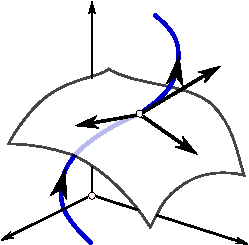
\includegraphics[width=\unitlength]{A28tangent3}}%
    \put(0.91612064,0.70682767){\color[rgb]{0,0,0}\makebox(0,0)[lb]{\smash{$\vel$}}}%
    \put(0.48698745,0.90266503){\color[rgb]{0,0,0}\makebox(0,0)[lb]{\smash{$\ssp(\zeit)$}}}%
    \put(0.2624318,0.5347756){\color[rgb]{0,0,0}\makebox(0,0)[lb]{\smash{$\groupTan_1$}}}%
    \put(0.80471037,0.38188675){\color[rgb]{0,0,0}\makebox(0,0)[lb]{\smash{$\groupTan_2$}}}%
    \put(0.538343,0.25344355){\color[rgb]{0,0,0}\makebox(0,0)[lb]{\smash{$\LieEl\ssp$}}}%
    \put(0.47864531,0.56060893){\color[rgb]{0,0,0}\makebox(0,0)[lb]{\smash{$\ssp$}}}%
  \end{picture}%
~~(b)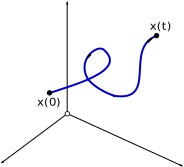
\includegraphics[width=0.20\textwidth]{A27traj}
\\
(c)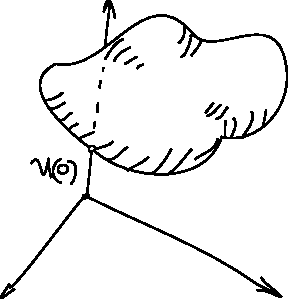
\includegraphics[width=0.20\textwidth]{A27gOrbit}
(d)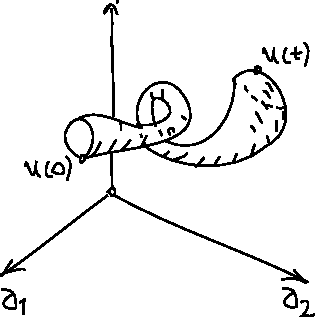
\includegraphics[width=0.20\textwidth]{A27wurst}
   \caption{\label{fig:A27wurst}
   (a)
In presence of $N$-continuous parameter symmetry, each \statesp\ point
$\ssp$ owns $(N\!+\!1)$ tangent vectors: one $\vel(\ssp)$ along the time
flow $\ssp(\zeit)$, and the $N$ group tangents  $\groupTan_1(\ssp), \,
\groupTan_2(\ssp) ,\,\cdots, \groupTan_N(\ssp)$ along infinitesimal
symmetry shifts, tangent to the group orbit $\LieEl\ssp$.
    (b)
Trajectory.
    (c)
Group orbit.
    (d)
Wurst.
}
\end{figure}
%%%%%%%%%%%%%%%%%%%%%%%%%%%%%%%%%%%%%%%%%%%%%%%%%%%%%%%%%%%%%%%%%%%%%

A flow $\map^t$ and the \statesp\ $\pS$ on which the flow acts comprise a
{dynamical system}. If a group $\Group$ of continuous transformations
acts on a continuous time flow, each \statesp\ point owns a set of
tangent vectors (\reffig{fig:A27wurst}\,(a)). Integrated globally, the
velocity vector $\vel(\ssp)$ traces out the {\em trajectory}
$\flow{\zeit}{\ssp}$ ( \reffig{fig:A27wurst}\,(b)). Applying the continuous
transformations traces out the {group orbit} (or, from now on, just
\emph{orbit})
\(
\pS_\ssp = \{\LieEl\,\ssp \mid \LieEl \in {\Group}\}
% \,,\qquad \pS_\ssp \subset \pS
\,
\) %ee{sspOrbit}
(\reffig{fig:A27wurst}\,(c)). Together they trace out a complicated smooth
manifold (hereafter affectionately referred to as the {\em wurst}, see
figures~\ref{fig:A27wurst}\,(d), \ref{fig:CLf01group}\,(b) and
\ref{fig:sliceimage}), that we shall teach you here how to slice.

A flow is said to have symmetry $\Group$ if the form of evolution
equations $\dot{\ssp} = \vel(\ssp)$ is left invariant,
\(
\vel(\ssp)=\LieEl^{-1} \, \vel(\LieEl \, \ssp)
% \,,\qquad \mbox{for all }
\,,
\) %ee{eq:FiniteRot}
by the set of transformations $\LieEl \in {\Group}$. Physicists love
symmetry, but Nature does not care: turbulence breaks all symmetries,
and while the flow equations may be invariant under $\Group$, their
solutions typically are not.

The key to chaotic dynamics is the notion of recurrence. To quantify how
close the state of the system now is to a previously visited state, we
need the notion of distance between two points in \statesp. The simplest
(but far from the only, or the most natural) is the Euclidean norm
\beq
  \Norm{\ssp-\ssp'}^2  = \braket{\ssp-\ssp'}{\ssp-\ssp'} =
\sum_j^d
(\ssp-\ssp')_j^2
\,.
\ee{innerproduct}
Given a notion of distance we can talk about 'neighborhood,' the open set of
nearby states. Our main task in what follows will be to make this precise,
by defining a chart over a neighborhood, and its borders.
Given distances and neighborhoods,
the next key notion is  \emph{measure}, or how likely a typical
trajectory is to visit a given neighborhood. After some observations of a
given turbulent flow, one can identify a set of representative
\emph{\template s}\rf{rowley_reconstruction_2000}, {points}
$\slicep{}^{(j)}$, $j=1,2,\cdots$ in the \statesp\ $\pS$, which are the
dynamically most important unstable {\recurrStr s} of the flow.
%    \DB{2012-04-12}{Neighborhoods not defined up to this point
%    in the text. Should they be? Predrag: done now.}

Our goals here are two-fold:
(i) In \refsect{s:cut} we review the method of Poincar\'e sections, with
    emphasis on aspects applicable to high-dimensional flows: construction of
    multiple local linear `charts' and determination of their borders and
(ii) in \refsect{s:slice} we show how the same set of tools applied to
    reduction of continuous symmetries enables us to commence a
    systematic charting of the long-time dynamics of high-dimensional
    flows with continuous symmetries (\refsect{s:chart}).

    \ifdraft\color{blue}
still to discuss:
\begin{itemize}

  \item section {\PoincS} vs slice \pSRed

  \item
dynamical system $\{\pS,\map^t\}$ with symmetry \Group\ vs reduced dynamics
$\{\pSRed,\mapRed^t\}$
  \item strobing $\sim$ method of connections
  \item reduction vs projection
\end{itemize}
    \color{black}\fi
